\documentclass[a4paper,12pt]{book} % nie: report!


\usepackage[T1,plmath]{polski} % lepiej to zamiast babel!
\usepackage[utf8]{inputenc} % w razie kłopotów spróbować: \usepackage[utf8x]{inputenc}
\usepackage{fancyhdr} % nagłówki i stopki
\usepackage{indentfirst} % WAŻNE, MA BYĆ!
\usepackage[pdftex]{graphicx} % to do wstawiania rysunków
\usepackage{amsfonts} % pakiety od AMS, ułatwiają składanie pewnych techniczno-matematcyznych rzeczy
\usepackage{amsmath} % to do dodatkowych symboli, przydatne
\usepackage{amssymb} % to też do dodatkowych symboli, też przydatne
\usepackage{amsthm}
\usepackage{enumitem}
\usepackage[pdftex,
            left=1.1in,right=1.1in,
            top=1.1in,bottom=1.1in]{geometry} % marginesy
\usepackage{float}
\usepackage[font=small,labelfont=bf]{caption}
\usepackage{svg}
\usepackage{booktabs}
\usepackage{array}
\usepackage{adjustbox}


\usepackage{csquotes}
\usepackage[backend=biber, style=numeric, citestyle=numeric]{biblatex}
\addbibresource{../bibliografia.bib}

\usepackage[colorlinks=true]{hyperref} % odnośniki interaktywne w PDFie
\hypersetup{allcolors=blue}

\usepackage{listings}
\lstset{
    basicstyle=\footnotesize\tt,
    numbers=left,
    numberstyle=\tiny,
    frame=tb,
    tabsize=4,
    columns=fixed,
    showstringspaces=false,
    showtabs=false,
    keepspaces,
    commentstyle=\color{red},
    keywordstyle=\color{blue}
}
\newfloat{lstfloat}{htbp}{lolst}[chapter]
\floatname{lstfloat}{Listing}
\def\lstfloatautorefname{Listing}


\pagestyle{fancy}
\renewcommand{\chaptermark}[1]{\markboth{#1}{}}
\renewcommand{\sectionmark}[1]{\markright{\thesection\ #1}}
\fancyhf{}
\fancyhead[LE,RO]{\footnotesize\bfseries\thepage}
\fancyhead[LO]{\footnotesize\rightmark}
\fancyhead[RE]{\footnotesize\leftmark}
\renewcommand{\headrulewidth}{0.5pt}
\renewcommand{\footrulewidth}{0pt}
\addtolength{\headheight}{1.5pt}
\fancypagestyle{plain}{\fancyhead{}\cfoot{\footnotesize\bfseries\thepage}\renewcommand{\headrulewidth}{0pt}}

\linespread{1.25}



\begin{document}
\begin{titlepage}
~

\begin{tabular}{c@{\hspace{21mm}}|@{\hspace{5mm}}l}
\vspace{-20mm} & \\
\multicolumn{2}{l}{\hspace{-12.5mm} \includegraphics[width=8cm]{assets/LogoUMCS.jpg}} \\
\multicolumn{2}{@{\hspace{20mm}}l}{\vspace{-4mm}} \\
\multicolumn{2}{@{\hspace{28mm}}l}{\Large \sf UNIWERSYTET MARII
	CURIE-SKŁODOWSKIEJ} \\
\multicolumn{2}{@{\hspace{28mm}}l}{\vspace{-4mm}} \\
\multicolumn{2}{@{\hspace{28mm}}l}{\Large \sf W LUBLINIE} \\
\multicolumn{2}{@{\hspace{28mm}}l}{\vspace{-4mm}} \\
\multicolumn{2}{@{\hspace{28mm}}l}{\Large \sf Wydział Matematyki, Fizyki i
	Informatyki} \\
\multicolumn{2}{@{\hspace{28mm}}l}{\vspace{21mm}} \\
& {\sf Kierunek: \textbf{informatyka} } \\
& \\\\\\
& {\sf \large \bfseries Rafał Lenart} \\
& {\sf nr albumu: 307726} \\
& \\\\\\
& \Large \sf \bfseries Porównanie wydajności i ocena\\
& \Large \sf \bfseries łatwości użycia wybranych narzędzi\\
& \Large \sf \bfseries programowania równoległego \\\\[-10pt]
& {\large \sf Performance comparison and} \\
& {\large \sf ease of use assessment} \\
& {\large \sf of selected parallel programming tools} \\
& \\
& \\
& \\
& {\sf Praca licencjacka}  \\
& \vspace{-7mm} \\
&  {\sf napisana w Katedrze cyberbezpieczeństwa i lingwistyki komputerowej} \\
& \vspace{-7mm} \\
&  {\sf Instytutu Informatyki UMCS} \\
& \vspace{-7mm} \\
& {\sf pod kierunkiem \bfseries dr. hab. Jarosława Byliny} \\
\multicolumn{2}{@{\hspace{28mm}}l}{\vspace{15mm}} \\
\multicolumn{2}{@{\hspace{28mm}}l}{\textbf{\textsf{Lublin 2024}}}
\end{tabular}
\end{titlepage}





\sloppy



\thispagestyle{empty}


\newpage{}

\thispagestyle{empty}

\newpage{}



\tableofcontents{}

\chapter*{Wstęp}
\addcontentsline{toc}{chapter}{Wstęp}

Tu treść wstępu

\chapter{Programowanie równoległe}


\section{Architektury komputerów równoległych}


\subsection{Taksonomia Flynna}
Taksonomia Flynna to klasyfikacja systemów komputerowych zaproponowana przez Michaela J. Flynna w 1996 roku \cite{Flynn1966}. System klasyfikacji uwzględnia jako czynniki liczbę strumieni rozkazów oraz liczbę strumieni danych.
W pierwotnej wersji Flynn opisał cztery klasy systemów komputerowych. Zaliczają się do nich:
\begin{itemize}[topsep=1pt, itemsep=0.5pt]
	\item Pojedynczy strumień rozkazów, pojedynczy strumień danych (ang. \emph{single instruction, single data, SISD}).
	\item Pojedynczy strumień rozkazów, wiele strumieni danych (ang. \emph{single instruction, multiple data, SIMD}).
	\item Wielokrotny strumień rozkazów, pojedynczy strumień danych (ang. \emph{multiple instruction, single data, MISD}).
	\item Wielokrotny strumień rozkazów, wiele strumieni danych (ang. \emph{multiple instruction, multiple data, MIMD}).
\end{itemize}
\newpage

\subsubsection{SISD}
W grupie SISD znajdują się komputery sekwencyjne, nie wykorzystujące zrównoleglenia w strumieniu danych, ani w strumieniu rozkazów. Pojedyncza jednostka sterująca przetwarza jeden strumień danych jednym rozkazem. W tej grupie znajdują się komputery w architekturze von Neumanna \cite{Neumann}. Przykładem systemów SISD mogą być wczesne komputery wykorzystujące jeden procesor (z jednym rdzeniem) do wykonywania wszystkich operacji.
\begin{figure}[h]
	\centering
	\includegraphics[scale=0.7]{assets/SISD.pdf}
	\caption{Diagram SISD}
	\label{SISD}
\end{figure}

\subsubsection{SIMD}
W komputerach z kategorii SIMD instrukcje mogą być wykonywane sekwencyjne lub równolegle przez kilka jednostek funkcyjnych. W artykule Flynna z roku 1972 \cite{Flynn1972} został dokonany podział klasy na trzy podkategorie:
\begin{itemize}
	\item Procesor wektorowy (ang. \emph{Array processor}) - obliczenia są wykonywane na całych wektorach danych, każda jednostka obliczeniowa posiada własny rejestr pamięci.
	\item Procesor potokowy (ang. \emph{Pipelined processor}) - jednostka obliczeniowa wykonuje instrukcje na fragmencie danych z centralnej jednostki pamięci i przetworzone dane zapisuje do tej samej jednostki.
	\item Procesor asocjacyjny (ang. \emph{Associative processor}) - tego typu systemy otrzymują ten sam rozkaz, jednak każda jednostka obliczeniowa podejmuje niezależną decyzję odnośnie tego czy wykonać zadaną instrukcję, czy ją pominąć. Decyzja ta jest podejmowana na podstawie danych otrzymanych przez daną jednostkę.
\end{itemize}
Superkomputery wektorowe były głównymi reprezentantami kategorii SIMD. Bardzo popularnym przykładem jest Cray-1 \cite{Cray-1}, superkomputer z lat siedemdziesiątych który obecnie znajduje się w Muzeum Nauki w Londynie. W wielu współczesnych architekturach procesorów są dostępne instrukcje które wykonują operacje wektorowe.
\begin{figure}[h]
	\centering
	\includegraphics[scale=0.7]{assets/SIMD.pdf}
	\caption{Diagram SIMD}
	\label{SIMD}
\end{figure}
\newpage

\subsubsection {MISD}
MISD jest architekturą stosowaną niezwykle rzadko, gdyż jedynym jej zastosowaniem jest minimalizacja błędów poprzez wykonywanie tej samej instrukcji wielokrotnie. Dobrze znanym przypadkiem użycia jest komputer Wahadłowca Kosmicznego skonstruowanego przez NASA \cite{SpaceShuttle}.
\begin{figure}[h]
	\centering
	\includegraphics[scale=0.7]{assets/MISD.pdf}
	\caption{Diagram MISD}
	\label{MISD}
\end{figure}

\subsubsection {MIMD}
MIMD to architektura pozwalająca na wykonywanie wielu instrukcji na wielu strumieniach danych. Jest to obecnie najbardziej popularna klasa komputerów. Nowoczesne komputery osobiste najczęściej posiadają wielo-rdzeniowe procesory które mają możliwość równoległego wykonywania różnych instrukcji na róznych zestawach danych.
\begin{figure}[h]
	\centering
	\includegraphics[scale=0.7]{assets/MIMD.pdf}
	\caption{Diagram MIMD}
	\label{MIMD}
\end{figure}

\newpage
\subsection{Pamięć komputera}
W systemach równoległych istnieją dwa modele organizacji pamięci:
\begin{itemize}
	\item Pamięć wspólna - wszystkie procesory w tym modelu mają dostęp do wspólnej przestrzeni adresowej. To rozwiązanie często może być wolniejsze poprzez jednoczesne próby dostępu do pamięci przez poszczególne jednostki. Dużą zaletą tego typu architektury jest łatwa komunikacja pomiędzy procesorami.
	\item Pamięć rozproszona - każdy z procesorów w tym modelu posiada pamięć lokalną, a komunikacja między nimi zachodzi przez sieć. Zaletą tego rozwiązania jest duża skalowalność oraz brak problemu jednoczesnego dostępu do pamięci. Niestety, niedogodnością jest konieczność stosowania bardziej skomplikowanych mechanizmów komunikacji oraz często wyspecjalizowanych algorytmów stworzonych dokładnie do tego celu. Projekt przykłada dużą uwagę do rozwiązań umożliwiających wykorzystanie pamięci rozproszonej używając standardu MPI oraz biblioteki distributed-ranges.
\end{itemize}
Duże znaczenie we współczesnych systemach komputerowych odgrywają również różne rodzaje pamięci.
\begin{itemize}
	\item Pamięć masowa/drugorzędna - pamięć długoterminowa zachowująca stan nawet po odłączeniu od źródła zasilania. Jest to najbardziej pojemny, ale i najwolniejszy rodzaj pamięci. W większości przypadków fizycznie znajduje się najdalej od procesora.
	\item Pamięc operacyjna, pamięć o dostępie swobodnym (ang. \emph{Random Access Memory}, RAM) - rodzaj pamięci znajdujący się niedaleko procesora, aby umożliwić duże prędkości przesyłu danych. Ma mniejszą pojemność niż pamięć masowa.
	\item Pamięć podręczna (ang. \emph{Cache memory}) - najszybsza pamięć, która przechowuje dane aktualnie przetwarzane przez procesor, fizycznie często jest zintegrowana bezpośrednio z procesorem. Ma ona małą pojemność.
\end{itemize}
W dzisiejszych czasach, rodzajem pamięci decydującym o prędkości wykonywanych operacji jest pamięć podręczna. Algorytmy oraz struktury danych, z których korzysta program, powinny być dobierane tak, aby zminimalizować konieczność częstego przenoszenia danych z RAM do pamięci podręcznej.
\begin{figure}[h]
	\centering
	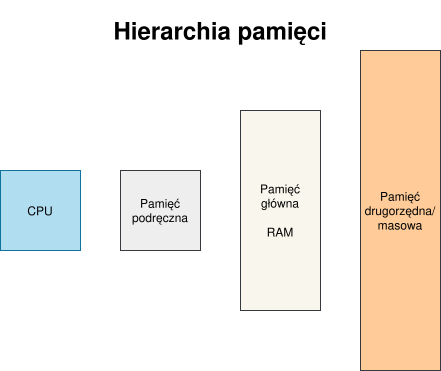
\includegraphics[scale=0.9]{assets/hierarchia_pamieci.pdf}
	\caption{Hierarchia pamięci}
	\label{hierarchia_pamieci}
\end{figure}

\chapter{Przegląd wykonanych testów}
\section{Wybrane narzędzia}
Narzędzia, które zostały wybrane do porównania to SYCL, MPI (ang. \emph{Message Passing Interface}) oraz biblioteka distributed-ranges wykorzystująca obydwie te technologie \cite{SYCL, MPI, dist-ranges}. Narzędzie przygotowane przez jeden z zespołów firmy Intel jako cel obrało zwiększenie produktywności pracy programistów przy pisaniu kodu. Chęć sprawdzenia obecnego stanu rozwoju tego narzędzia skłoniła mnie do jego wyboru. MPI oraz SYCL zostały wybrane ze względu na to, że distributed-ranges w dużej mierze bazuje na tych dwóch technologiach.
\subsection{SYCL}
Na stronie internetowej grupy Khronos, twórców narzędzia, widnieje zdanie ,,SYCL to bezpłatna, wieloplatformowa warstwa abstrakcji [...]''\cite{SYCL-overview}. Jest on modelem zgodnym ze standardem C++ 17. Jego zadaniem i głównym celem jest umożliwienie współpracy wielu urządzeniom w jednej aplikacji. Twórcom udaje się to poprzez udostępnienie API (ang. \emph{Application Programming Interface}, interfejsów programistycznych aplikacji) oraz abstrakcji dających dostęp do urządzeń takich jak procesory, karty graficzne czy FPGA (ang. \emph{Field Programmable Gate Array}, bezpośrednio programowalne macierze bramek). SYCL jest więc modelem wysoko-poziomowym, używającym nowoczesnych standardów, który upraszcza działanie z wieloma urządzeniami na raz. Wstępna specyfikacja SYCL została udostępniona 19 marca 2014 roku \cite{SYCL1.2-provisional}. Finalna specyfikacja SYCL 1.2 była wydana ponad rok później 11 Maja 2015 roku \cite{SYCL1.2}. Obecnie najnowszym wydaniem specyfikacji jest SYCL 2020 z 9 Lutego 2021 roku. Istnieje kilka rozwijanych równolegle implementacji modelu SYCL. Ja zdecydowałem się na użycie rozwiązania firmy Intel zawartego w zestawie narzędzi oneAPI. Podczas pracy nad projektem korzystałem z
\subsection{MPI}
Interfejs przekazywania wiadomości (ang. \emph{Message Passing Interface}, MPI) jest standardem przekazywania wiadomości pomiędzy  procesami programów równoległych. Ten protokół komunikacyjny utworzony i ustandaryzowany w czerwcu roku 1994 roku jest rezultatem prac wielu osób oraz firm. MPI jest szeroko wykorzystywany przy tworzeniu programów działających w systemach z pamięcią rozproszoną. Wiele języków programowania posiada własne implementacje MPI, jednak najczęściej używanymi są kompilatory języków C, C++ oraz Fortran. Standard od czasu swojego powstania był wciąż rozwijany i powstało kilka wersji, które bazowały i wzbogacały swoich poprzedników o nowe funkcje. Najnowszą zatwierdzoną przez forum wersją jest MPI-4.1 z listopada roku 2023 \cite{mpi41}.
\subsection{Distributed Ranges}
Zakresy rozproszone (ang. \emph{Distributed Ranges}) to biblioteka języka C++ utworzona przez firmę Intel zwiększająca produktywność pracy w systemach z pamięcią rozproszoną. Narzędzie to wykorzystuje bibliotekę ranges ze standardu C++ 20 i oferuje kolekcję struktur danych, widoków oraz algorytmów. Distributed ranges jest kompatybilna i zdolna do współpracy z MPI, SYCL, OpenMP oraz SHMEM. Kod źródłowy biblioteki jest otwarty i dostępny za darmo \cite{dist-ranges}. Repozytorium powstało i jest rozwijane od roku 2022. Jako, że zarówno biblioteka ranges (C++ 20) jak i distributed-ranges są technologiami wprowadzonymi niedawno, postaram się przybliżyć najważnejsze informacje z nimi związane.
\subsubsection{Ranges}
Nagłówek \emph{<ranges>} zawiera kilka konceptów (ang. \emph{concept}) które są, w najprostszej swojej postaci, abstrakcją dowolnego, iterowalnego zbioru elementów posiadającego początek i koniec \cite{ranges}. kolekcja ta, aby spełnić bazową definicję \emph{range}, musi posiadać metody \emph{begin()} oraz \emph{end()}. W tabeli \ref{ranges_concepts} znajduje się krótki opis kilku konceptów z \emph{std::ranges} oraz informacja o tym które z najczęściej używanych struktur danych z STL (ang. \emph{Standard Template Library}, Standardowa biblioteka szablonów) spełniają dany koncept.
\begin{table}[H]
\begin{adjustbox}{max width=\textwidth}
\begin{tabular}{|l|m{7cm}|ccccc|}
\hline
	& Opis & \texttt{std::forward\_list} & \texttt{std::list} & \texttt{std::deque} & \texttt{std::array} & \texttt{std::vector} \\
\hline
\texttt{std::ranges::output\_range} & Może iterować do przodu & X & X & X & X & X \\
\hline
\texttt{std::ranges::input\_range} & Można iterować po nim od początku do końca przynajmniej raz & X & X & X & X & X \\
\hline
\texttt{std::ranges::forward\_range} & Można iterować po nim od początku do końca wielokrotnie & X & X & X & X & X \\
\hline
\texttt{std::ranges::bidirectional\_range} & Iterator może poruszać się do tyłu & & X & X & X & X \\
\hline
\texttt{std::ranges::random\_access\_range} & Dostęp do każdego elementu jest w czasie stałym & & & X & X & X \\
\hline
\texttt{std::ranges::contiguous\_range} & Elementy są przechowywane w pamięci jeden po drugim & & & & X & X \\
\hline
\end{tabular}
\end{adjustbox}
\caption{Wybrane koncepty z std::ranges}
\label{ranges_concepts}
\end{table}
W bibliotece zdefiniowane są klasy widoków (ang. \emph{view}). Widok to zakres odwołujący się do elementów, których nie posiada. Widok jest sposobem modyfikacji zakresu, do którego się odwołuje. Łączenie i tworzenie widoków jest bardzo wydajne, gdyż uzyskiwanie dostępu do elementów widoku odbywa się "leniwie", czyli tak, aby operacje zostały wykonane dopiero przy próbie dostępu do wartości. Przykładem wykorzystania zakresów może być Listing \ref{lst:ranges_przyklad}. Jak widać, widoki można łączyć ze sobą aby w prosty i wydajny sposób wykonywać większe, bardziej skomplikowane operacje. Odbywa się to często poprzez użycie operatora potoku ("$|$") znanego na przykład z powłoki Bash.

\begin{lstfloat}[H]
\lstset{language=C++}
\begin{lstlisting}[frame=single]
#include <ranges>
#include <vector>
#include <iostream>

int main() {
	std::vector<int> input =  {0, 1, 2, 3, 4, 5, 6, 7, 8, 9};
    auto is_even = [](const int val) {return val % 2 == 0;};
    auto times_two = [](const int val) {return val * 2;};

    auto result = input
             | std::views::filter(is_even)
             | std::views::transform(times_two);
    
    std::cout << "Wynik: ";
    for (int val : result) {
    		std::cout << val << ' ';
  	}
}

Wynik: 0 4 8 12 16
\end{lstlisting}
\caption{Przykład użycia biblioteki \emph{ranges}}\label{lst:ranges_przyklad}
\end{lstfloat}

\subsubsection{Distributed Ranges}
Podobnie jak opisana wyżej biblioteka z C++ 20, distributed ranges wprowadza kilka konceptów na których bazowane są struktury. Najważniejszym z tych konceptów jest \texttt{distributed\_range} opisany tak jak na listingu \ref{lst:distributed_range} w pliku \emph{concepts.hpp}.

\begin{lstfloat}[H]
\lstset{language=C++}
\begin{lstlisting}[frame=single]
template <typename R>
concept distributed_range =
  rng::forward_range<R> && requires(R &r) { dr::ranges::segments(r); };
\end{lstlisting}
\caption{Koncept \texttt{distributed\_range}}
\label{lst:distributed_range}
\end{lstfloat}

Ponadto, biblioteka jest podzielona na dwie przestrzenie nazw czyli \texttt{dr::mhp} oraz \texttt{dr::shp}. Na potrzeby mojego projektu bardziej interesującą częścią biblioteki jest zdecydowanie mhp. Udostępnia ona dwie struktury danych \texttt{dr::mhp::distributed\_vector} oraz \texttt{dr:mhp::distributed\_dense\_matrix}. Udostępnione dla tych struktur operacje mogą być wykorzystywane do programowania systemów komputerowych z pamięcią rozproszoną poprzez użycie połączenia MPI oraz SYCL. Druga część biblioteki pozwala, tak jak mhp oraz SYCL, na wykorzystanie kilku CPU/GPU, jednak w jednym procesie i tylko na jednym węźle. Niestety \texttt{dr::shp} jest bardziej rozwinięta i posiada więcej funkcji oraz narzędzi które jeszcze nie zostały zaimplementowane w mhp. Dla obu części istnieje obecnie zbiór widoków pozwalających na przeprowadzanie operacji w sposób identyczny jak w \texttt{<ranges>}.




\section{Wybrane algorytmy}
\subsection{Całkowanie metodą Monte Carlo}
Metodami Monte Carlo nazywamy techniki i algorytmy uzyskiwania wyników operacji numerycznych poprzez wielokrotne losowe próbkowanie. Głównym twórcą metody był polski fizyk Stanisław Ulam, który zainspirowany hazardowymi nawykami swojego wójka nadał jej nazwę pochodzącą od kasyna Monte Carlo w Monako.\cite{mc_beggining}
Obliczanie całki tą metodą to bardzo prosta operacja. Wystarczy wylosować dostateczną ilość punktów z podanego zakresu aby zapewnić wysoką dokładność wyniku i dla każdego z nich sprawdzić czy znajduje się on pod wykresem sprawdzanej funkcji. Dokładność wyników otrzymanych przez użycie tej metody zależy w dużej mierze od parametrów wybranego generatora liczb pseudolosowych.
W projekcie zdecydowałem się na obliczanie całki wielowymiarowej, co sprowadza się do obliczenia objętości pod funkcją. Jako zakres całkowania przyjąłem hipersześcian współdzielącym środek z układem współrzędnych. Zdecydowałem się na taki zabieg po to, aby zwiększyć ilość obliczeń, a tym samym czas wykonywania programu.
\subsection{Metoda gradientu sprzężonego}
Metoda gradientu sprzężonego (ang. \emph{conjugate gradient method}, CG) jest metodą numeryczną zaproponowaną w 1952 roku \cite{conjugate-gradient}, pozwalającą na rozwiązywanie układów równań liniowych, których macierz $A$ spełnia następujące warunki:
\begin{itemize}
\item jest symetryczna $A^T=A,$
\item jest dodatnio określona.
\end{itemize}

Dwa niezerowe wektory $u$ i $v$ są sprzężone względem macierzy $A,$ jeśli $u^TAv=0.$ Ponadto, sprzężoność jest relacją symetryczną. To oznacza, że jeśli $u$ jest sprzężony z $v,$ to $v$ jest sprzężony z $u$.
\\
Załóżmy, że $P = {p_1,...,p_n}$ jest zbiorem sprzężonych ze sobą, względem macierzy $A,$ wektorów, czyli $p_i^TAp_j = 0$ dla wszystkich $i \neq j$. Wtedy rozwiązaniem $x_\ast$ układu $Ax=b$ jest 
$$ x_\ast = \sum_{i=1}^n\alpha_ip_i \Rightarrow Ax_\ast = \sum_{i=1}^n\alpha_iAp_i. $$
Współczynniki możemy znaleźć wtedy poprzez przemnożenie równania $Ax=b$ przez wektor $p_k^T,$ co daje:
$$ p_k^TAx_\ast = \sum_{i=1}^n\alpha_ip_k^TAp_i = p_k^Tb $$
$$ \alpha_k = \frac{p_k^Tb}{p_k^TAp_k} $$
Dodatkowo, dzięki temu że $A$ jest symetryczna i dodatnio określona możemy zapisać, że
$$\langle u, v\rangle_A := \langle A^Tu, v\rangle = \langle Au, v\rangle = \langle u,Av\rangle = u^TAv.$$
$$ \alpha_k = \frac{p_k^Tb}{p_k^TAp_k} = \frac{\langle p_k, b \rangle}{\langle p_k, p_k\rangle _A} = \frac{\langle p_k, b\rangle}{||p_k||_A^2}$$
Uzyskujemy przez to metodę rozwiązywania $Ax = b.$ Najpierw należy znaleźć ciąg sprzężonych kierunków, a następnie obliczyć współczynniki $\alpha_k.$
\\

CG jest metodą iteracyjną. Jest tak dlatego, że odpowiedni dobór sprzężonych wektorów $p_k$ zwykle sprawia, że nie potrzebujemy ich wszystkich do dobrego przybliżenia wyniku. Dzięki temu metoda gradientu sprzężonego pozostaje wydajna nawet dla bardzo dużych macierzy.
Dla większości przypadków punkt startowy $x_0 = 0$. Zauważmy, że rozwiązanie $x_\ast$ minimalizuje formę kwadratową:
$$ f(x) = \frac{1}{2}x^TAx-x^Tb, x\in R^n.$$
To skłania nas do wybrania do roli pierwszego wektora bazowego $p_0,$ odwrotności gradientu $f$ w $x = x_0,$ która wynosi $b.$ Nazwa metody bierze się z faktu, że pozostałe wektory będą sprzężone do tego gradientu.

Niech $r_k$ oznacza rezyduum w k-tym kroku:
$$r_k = b-Ax_k.$$ Jako, że zakładamy wzajemną sprzężoność kierunków $p_k,$ wybieramy kierunek najbliższy do $r_k.$\cite{cg_wiki}
$$p_{k+1} = r_k - \frac{p_k^TAr_k}{p_k^TAp_k}p_k$$
Bardzo przydatną publikacją wyjaśniającą z większą ilością szczegółów metodę gradientu sprzężonego jest praca Jonathana R. Shewchuka z 1994 roku \cite{cg_without_pain}. W tym dokumencie autor oblicza złożoność obliczeniową algorytmu jako $O(m\sqrt{k}),$ gdzie $m$ to liczba niezerowych wpisów w $A,$ a $k$ jest wskaźnikiem uwarunkowania.

Zgodnie z powyższym opisem metody, zapisałem algorytm rozwiązujący $Ax = b$ metodą gradientu sprzężonego w postaci kodu języka Python. Znajduje się on w listingu \ref{lst:cg_python}. Funkcja dla podanej symetrycznej, dodatnio określonej macierzy $A$, oraz wektora $b$ zwraca wynikowy wektor $X$ z podaną tolerancją błędu przybliżenia.

\begin{lstfloat}[H]
\lstset{language=Python}
\begin{lstlisting}[frame=single]
def conjugate_gradient(A, b, tolerance):
    X = np.zeros(len(b))
    residual = b
    search_dir = residual

    old_resid_norm = numpy.linalg.norm(residual)

    while old_resid_norm > tolerance:
        A_search_dir = np.dot(A, search_dir)
        alpha = old_resid_norm**2 / np.dot(search_dir, A_search_dir)
        X = X + alpha * search_dir
        residual = residual + -alpha * A_search_dir

        new_resid_norm = numpy.linalg.norm(residual)

        mod = (new_resid_norm/old_resid_norm)**2
        search_dir = search_dir * mod + residual
        old_resid_norm = new_resid_norm

    return X
\end{lstlisting}
\caption{Implementacja metody gradientu sprzężonego w języku Python}
\label{lst:cg_python}
\end{lstfloat}

\subsubsection{Potrzebne testowe dane wejściowe}
Metoda CG rozwiązuje układ równań liniowych w postaci $Ax = b.$ Danymi wejściowymi więc będzie macierz $A$ oraz wektor $b$. Generacja wektora nie sprawia żadnego problemu, w projekcie generowany wektor zawiera liczby rzeczywiste z przedziału od $0$ do $40,$ gdyż nie musi on spełniać żadnych szczególnych warunków.
Jako metodę generacji losowej macierzy symetrycznej, dodatnio określonej, przyjąłem następujący przepis.
\begin{enumerate}
		\item Wygenerowanie macierzy zawierającej losowe wartości rzeczywiste od $0$ do $1.$
		\item Przemnożenie wygenerowanej macierzy przez jej transpozycję $A * A^T,$ co gwarantuje symetryczność.
		\item Dodanie do wyniku poprzedniej operacji macierzy jednostkowej przemnożonej przez rozmiar macierzy. Ta operacja gwarantuje dodatnią określoność wynikowej struktury.
\end{enumerate}
Kod w języku Python realizujący ten sposób na generację $A$ znajduje się w listingu \ref{lst:gen_spd_matrix}. Jedyną daną wejściową \texttt{n} jest żądana wielkość macierzy.

\begin{lstfloat}[H]
\lstset{language=Python}
\begin{lstlisting}[frame=single]
def generate_spd_matrix(n):
    A = np.random.rand(n, n)
    B = np.dot(A, A.T)
    C = B + n * np.eye(n)

    return C
\end{lstlisting}
\caption{Funkcja generacji symetrycznej, dodatnio określonej macierzy w języku Python}
\label{lst:gen_spd_matrix}
\end{lstfloat}

\subsection{Szybka transformata Fouriera}
Transformata Fouriera to funkcja nazwana na cześć Jeana Baptiste'a Josepha Fouriera, francuskiego matematyka, który odkrył że dowolny sygnał okresowy może zostać przedstawiony w postaci szeregu Fouriera. Szeregiem Fouriera nazywamy sumę sygnałów trygonometrycznych o różnych amplitudach i częstotliwościach. Transformacja Fouriera to operacja przekształcająca sygnał z dziedziny czasu do dziedziny częstotliwości. Transformacje Fouriera są często wykorzystywane do kompresji danych dźwiękowych, obrazów i filmów. Przykładem zastosowania może być algorytm kompresji JPEG, ale istnieje mnóstwo innych, ważnych zastosowań.

DFT (ang. \emph{Discrete Fourier Transform}, Dyskretna transformata Fouriera) to rodzaj transformaty fouriera przyjmujący jako dane wejściowe sygnał próbkowany, a więc dyskretny. Transformatę określamy następującym wzorem: $$ {X_k = \sum_{n=0}^{N-1}x_n*e^{-i2\pi \frac{k}{N}n}},$$gdzie $ \{x_n\} := x_0, x_1, ..., x_{N-1} $ to ciąg $N$ liczb zespolonych zamieniany na ciąg wynikowy liczb zespolonych $ \{ X_k\} := X_0, X_1, ..., X_{N-1} $. Złożoność obliczeniowa obliczania DFT wynosi $O(n^2).$

Przez zwiększenie ilości danych wymagających analizy na przestrzeni lat, powstały algorytmy do obliczania tzw. FFT(ang. \emph{Fast Fourier Transform}, szybka transformata Fouriera). Tego typu operacje diametralnie zmniejszają złożoność obniżając ją z $O(n^2),$ znanego z DFT, do $O(nlog_2n).$ Osiągnięcie tak dobrego wyniku jest możliwe na przykład poprzez podział na podproblemy.
\subsubsection{Algorytm Cooleya-Tukeya}
Zwany również jako "Radix-2 FFT", algorytm Cooleya-Tukeya polega na rekurencyjnym dzieleniu problemu na mniejsze DFT dzieląc je na ciąg wpisów o indeksach parzystych i drugi o indeksach nieparzystych.\cite{CooleyTukey} Aby dokonać takiego podziału, wielkość wejściowego ciągu danych musi być potęgą liczby 2: $N = 2^n.$ Przypadkiem bazowym dla takiego podejścia jest ciąg o rozmiarze $N = 1.$

Biorąc pod uwagę potrzebę zrównoleglenia działań wykonywanych w przebiegu projektu, metoda rekurencyjna utrudniałaby produktywną pracę. Zdecydowałem się więc na przekształcenie metody w wersję iteracyjną. Aby to wykonać, ważnym działaniem jest odwrócenie bitowe indeksów w wektorze wejściowym, co ułoży je w sposób identyczny do tego, który uzyskałbym poprzez wielokrotny podział. Zjawisko to jest pokazane w tabeli \ref{tab:bit_reversal} w której zapisałem liczby z zakresu 0 do 7 odwrócone bitowo, oraz na rysunku \ref{fig:bit_reversal} który reprezentuje graficznie podział ciągu 8 liczb, tak jak miałoby to miejsce przy podejściu rekurencyjnym. Reprezentację algorytmu Cooleya-Tukeya w języku Python przedstawiłem w listingu \ref{lst:fft_python}.

\begin{table}[H]
\begin{adjustbox}{max width=\textwidth}
\begin{tabular}{|l|l|l|l|}
\hline
Indeks & Zapis binarny & Zapis binarny odwrócony bitowo & Indeks odwrócony bitowo \\
\hline
0 & 000 & 000 & 0 \\
1 & 001 & 100 & 4 \\
2 & 010 & 010 & 2 \\
3 & 011 & 110 & 6 \\
4 & 100 & 001 & 1 \\
5 & 101 & 101 & 5 \\
6 & 110 & 011 & 3 \\
7 & 111 & 111 & 7 \\
\hline
\end{tabular}
\end{adjustbox}
\caption{Odwrócenie bitowe}
\label{tab:bit_reversal}
\end{table}

\begin{figure}[h]
	\centering
	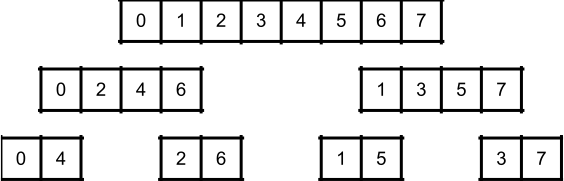
\includegraphics[scale=0.7]{assets/bit_reversal.pdf}
	\caption{Podział w kolejnych krokach rekurencyjnych}
	\label{fig:bit_reversal}
\end{figure}

\begin{lstfloat}[H]
\lstset{language=Python}
\begin{lstlisting}[frame=single]
def fft(input_arr):
    input_arr = reverse_array_with_bit_indices(input_arr)
    num_bits = int(np.ceil(np.log2(len(input_arr))))

    for step in range(1, num_bits+1):
        step_size = 1 << step
        omega = cmath.exp(-2j * math.pi / step_size)
        for start in range(0, len(input_arr), step_size):
            omega_power = 1
            for i in range(step_size // 2):
                index_even = start + i
                index_odd = start + i + step_size // 2
                temp = input_arr[index_even]
                input_arr[index_even] += (
                        omega_power * input_arr[index_odd])
                input_arr[index_odd] = (
                        temp - omega_power * input_arr[index_odd])
                omega_power *= omega

    return input_arr
\end{lstlisting}
\caption{Implementacja algorytmu Cooleya-Tukeya w języku Python}
\label{lst:fft_python}
\end{lstfloat}
\subsubsection{Potrzebne testowe dane wejściowe}
Do poprawnego działania algorytmu Cooleya-Tukeya potrzebny jest wektor o długości $N = 2^n,$ gdzie $n \in \mathbb{N}$. W projekcie użyłem wektora liczb zespolonych zawierającego liczby, których część rzeczywista jest losowana z przedziału 0 do 1.
\section{Przygotowanie środowiska}
Wszystkie testy oraz cała konfiguracja została wykonana na komputerze wyposażonym w 6-rdzeniowy, 12-wątkowy procesor AMD Ryzen 5 5600 z dostępem do 32 GB pamięci RAM.
Systemem operacyjnym zainstalowanym na komputerze jest Debian 12.
\subsection{Konfiguracja CMake}
W projekcie zostało użyte dobrze znane narzędzie do zarządzania procesem kompilacji programu "CMake". W przypadku programów sekwencyjnych oraz MPI nie korzystałem z CMake ponieważ nie było takiej potrzeby.
Dla SYCL bardzo wygodnym i przydatnym narzędziem była funkcja \texttt{CMAKE\_EXPORT\_COMPILE\_COMMANDS} na potrzeby programu clangd. W tym przypadku narzędzie zostało użyte w większości dla własnej wygody. Bardzo podstawowym przykładem zawartości pliku konfiguracyjnego \emph{CMakeLists.txt} może być ten zawarty w listingu \ref{lst::cmake-SYCL}

\begin{lstfloat}[H]
\begin{lstlisting}[frame=single]
cmake_minimum_required(VERSION 3.0)

set(CMAKE_CXX_COMPILER "icpx")
set(CMAKE_CXX_FLAGS "${CMAKE_CXX_FLAGS}-fsycl -O3 -std=c++17")
set(CMAKE_EXPORT_COMPILE_COMMANDS ON)

project(FFT_SYCL LANGUAGES CXX)
set(SOURCES 
    src/main.cpp
)

add_executable(main ${SOURCES})
\end{lstlisting}
\caption{Plik konfiguracyjny CMakeLists.txt rozwiązań używających SYCL}
\label{lst::cmake-SYCL}
\end{lstfloat}

Biblioteka Distributed Ranges przysporzyła pewnych kłopotów. Na dzień w którym przygotowywałem środowisko do użycia narzędzia, rozwiązanie z repozytorium projektu w serwisie GitHub nie działało poprawnie. Wziąłem więc przykład z pobocznego repozytorium zawierającego przykładowy projekt używający tej biblioteki. \cite{dist-ranges-tutorial}
\subsection{Użyte Kompilatory}
Kompilując programy spełniające sekwencyjne podejście do wybranych problemów użyta została Kolekcja Kompilatorów GNU (ang. \emph{GNU Compiler Collection}, GCC) dołączona w systemie Debian.

Bardzo ważną częścią konfiguracji jest zestaw narzędzi oneAPI udostępniany przez firmę Intel. Pozostałe kompilatory użyte do obsługi MPI, SYCL a także Distributed Ranges pochodzą z tej właśnie kolekcji. Poradnik instalacji paczki dla systemów z grupy GNU/Linux znajduje się pod adresem przypisanym do pozycji \cite{oneapi-install} z bibliografii. Koniecznym działaniem do zapewnienia poprawnego przygotowanych przeze mnie programów jest uruchomienie skryptu ustawiającego odpowiednie zmienne w powłoce. Domyślną ścieżką tego skryptu po instalacji zestawu oneAPI jest \emph{/opt/intel/oneapi/setvars.sh}.

Użyte kompilatory do poszczególnych narzędzi:
\begin{itemize}
\item Programy Sekwencyjne - \textbf{gcc/g++}
\item MPI - \textbf{mpicxx}
\item SYCL oraz Distributed Ranges - \textbf{icx/icpx}
\end{itemize}
Każdy z programów jest kompilowany używając flagi \emph{-O3} włączającej wszystkie optymalizacje.
\subsection{Inne narzędzia}
Narzędziem którego użyłem przy pisaniu był program Scalasca opisany w tym artykule \cite{scalasca}. Aplikacja służy do analizy przebiegu programów równoległych napisanych przy użyciu modeli MPI oraz Open-MP. Okazało się ono bardzo przydatne do wykrywania problemów z wydajnością dla moich implementacji w języku MPI.

Pragnę również wspomnieć o pewnym niezbyt istotnym, niemniej jednak niewygodnym, problemie który napotkałem próbując skonfigurować clangd, serwer językowy usprawniający pisanie kodu poprzez dodanie funkcjonalności do edytora tekstu takich jak uzupełnianie kodu czy szybki dostęp do definicji. Okazało się bowiem iż zestaw oneAPI zawiera własną wersję tego narzędzia, znajduje się ona pod ścieżką \emph{/opt/intel/oneapi/compiler/latest/bin/compiler/clangd}. Niestety podana kompilacja nie wykrywała poprawnie plików nagłówkowych zawartych we własnym zestawie co zmusiło mnie do własnoręcznej kompilacji narzędzia z odpowiednim kompilatorem (\texttt{icpx}).

W katalogu głównym projektu zamieściłem skrypt \emph{build\_all.sh} służący do kompilacji wszystkich plików źródłowych i zapisania ich w katalogu \emph{build/.}

\chapter{Problemy implementacyjne}
\section{Implementacja sekwencyjna}
\subsection{Przegląd krytycznych części programu}
\subsection{Ostateczny czas wykonania - komentarz}
\section{SYCL}
\subsection{Przegląd krytycznych części programu}
\subsection{Ostateczny czas wykonania - komentarz}
\section{MPI}
\subsection{Przegląd krytycznych części programu}
\subsection{Ostateczny czas wykonania - komentarz}
\section{distributed-ranges}
\subsection{Przegląd krytycznych części programu}
\subsection{Ostateczny czas wykonania - komentarz}

\chapter{Porównanie łatwości w użyciu}
W tym rozdziale zawieram subiektywną opinię opisaną z perspektywy osoby która po raz pierwszy używałą każdego z użytych narzędzi. Postaram się pominąć tutaj kwestię wydajności poszczególnych rozwiązań i skupić się jedynie na łatwości w użyciu.

Implementacja równoległych rozwiązań w MPI okazała się najtrudniejsza, co jest wynikiem przewidywalnym. MPI daje pełną kontrolę nad podziałem pamięci, i nad sposobem komunikacji pomiędzy poszczególnymi procesami. Przez to łatwo jest popełnić drobne, trudne do znalezienia błędy. Ilość napisanych linijek kodu jest o wiele większa od pozostałych rozwiązań. Model MPI wymaga dobrego zrozumienia oraz dużej wiedzy na temat poprawnych praktyk aby pisać kod dobrej jakości.

Pisanie kodu w SYCL jest w porównaniu do MPI dość przyjemne i szybkie. Model wymagał jednak pewnego rodzaju początkowego obeznania gdyż wprowadza wiele specyficznych metod tworzenia oprogramowania które nie są od początku intuicyjne. Jako dobre wprowadzenie do SYCL mogę polecić książkę \cite{sycl-book} która bardzo dobrze wyjaśnia zarówno podstawowe techniki jak i te bardziej zaawansowane. Narzędzie spodobało mi się na tyle, że skorzystałem z niego przy tworzeniu programów do generacji danych wejściowych zarówno dla metody gradientu sprzężonego jak i szybkiej transformaty Fouriera.

Distributed Ranges po raz kolejny jest dla mnie trudnym przypadkiem do opisania, braki w funkcjonalnościach przestrzeni nazw \emph{mhp} uniemożliwiają, w mojej opinii efektywne wprowadzenie biblioteki do jakiegokolwiek większego projektu. Wymusza to rodzaj pracy podobny do tego w MPI lecz bardziej ograniczony. Uważam jednak, że narzędzie ma duży potencjał. Funkcje które są obecnie zaimplementowane były bardzo łatwe i intuicyjne w użyciu. Praca ze strukturami prawie nie rózni się od pracy z biblioteką \emph{<ranges>} ze standardu C++20. Jednym wynikającym z równoległej natury biblioteki problemem jest brak możliwości przekazywania referencji do wyrażeń lambda używanych w pracy z widokami. Podobne zachowanie można zaobserwować w SYCL który jest eksploatowany przez Distributed Ranges. Jestem bardzo ciekawy jak potoczy się dalszy rozwój narzędzia i mam nadzieję że funkcjonalności z przestrzeni \emph{shp} takie jak funkcja mnożenia macierzy przez wektor znajdą się także w części \emph{mhp}

\chapter{Porównanie wydajności}
\section{Wykresy, zebrane dane}
\section{Wyjaśnienie}
\section{Wnioski}

\chapter{Podsumowanie}


\listof{lstfloat}{Spis listingów} % jeśli są listingi
\addcontentsline{toc}{chapter}{Spis listingów}

\listoftables{} % jeśli są tabele
\addcontentsline{toc}{chapter}{Spis tabel}

\listoffigures{} % jeśli są rysunki
\addcontentsline{toc}{chapter}{Spis rysunków}

\printbibliography

\end{document}
